\chapter{ГЛАВА 2 ИССЛЕДОВАНИЕ ТОЧНОСТИ КООРДИНАТ ПРИ ОБРАБОТКЕ СОВРЕМЕННЫМИ МЕТОДАМИ ОБРАБОТКИ ДАННЫХ }\label{ch:ch2}

На сегодняшний день обработка по РРР-алгоритму реализована несколькими способами. Во-первых, обработка может выполняться с использованием интернет-сервисов. Во-вторых, обработка может быть выполнена в коммерческих программных обеспечениях. В-третьих, существуют некоторые бесплатные (некоммерческие) программные обеспечения с открытым кодом.

В первой части главы рассмотрены современные способы обработки данных по РРР-алгоритму. Вторая часть главы посвящена исследованию точности определения координат по РРР-алгоритму при вариации различных факторов.

\section{Обзор современных сервисов для обработки РРР}\label{sec:ch2/sec1}

На сегодняшний день международным научным сообществом разработаны интернет-сервисы для обработки данных по РРР-алгоритму, обзор которых приведен ниже.

\subsection{Trimble RTX (Trimble RTX Post Processing)}\label{subsec:ch2/sec1/sub1}

Trimble RTX один из самых перспективных онлайн-сервисов для обработки спутниковых данных по РРР-алгоритму \cite{src81}. Точность определения координат варьируется от сантиметров и заканчивая субсантиметровым уровнем точности. Существует возможность предоставления обработанных координат, как в общеземной системе координат ITRF~2014 (на эпохи 2010 и 2024.25), так и в геодезической системе координат (BLH).

Основные сведения о данном интернет-сервисе: 
\begin{list}{$ \checkmark $\\[6pt]} {\parsep = \parskip \itemsep=\parsep \topsep=0em}
	\item Бесплатный сервис. 
	\item Существует возможность обрабатывать данные современных ГНСС.
	\item Минимальная продолжительность измерений необходимая для обработки составляет 10 минут; максимальная суточный файл.
	\item RINEX файл или фирменные файлы должны содержать только данные собранные двух-частотным спутниковым приемником и только в статике.
	\item Отсутствует возможность обработки только данных ГЛОНАСС.
\end{list}

\begin{itemize}
	\item Бесплатный сервис. 
	\item Существует возможность обрабатывать данные современных ГНСС.
	\item Минимальная продолжительность измерений необходимая для обработки составляет 10 минут; максимальная суточный файл.
	\item RINEX файл или фирменные файлы должны содержать только данные собранные двух-частотным спутниковым приемником и только в статике.
	\item Отсутствует возможность обработки только данных ГЛОНАСС.
\end{itemize}

На рисунке \cref{fig:pic06} представлен фрагмент интерфейса данного интернет-сервиса.

\begin{figure}[h]
	\centering
	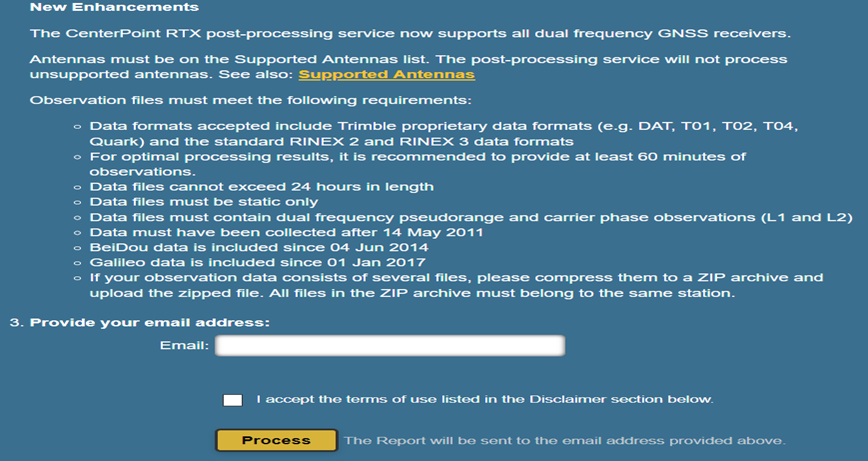
\includegraphics[width=\linewidth]{images/pic06}
	\caption{Интерфейс сайта Trimble RTX}
	\label{fig:pic06}
\end{figure}

При обработке с использованием данного интернет-сервиса необходимо загрузить обрабатываемый RINEX-файл либо фирменный формат Trimble (T01, T02, T03, T04). Далее выбирается литосферная плита, либо указывается автоматически в процессе обработки. Затем указывается электронная почта, на которую придет обработанный файл в формате pdf. На рисунке \cref{fig:pic07} приведен пример отчета по обработке с использованием данного интернет-сервиса.

\begin{figure}[h]
	\centering
	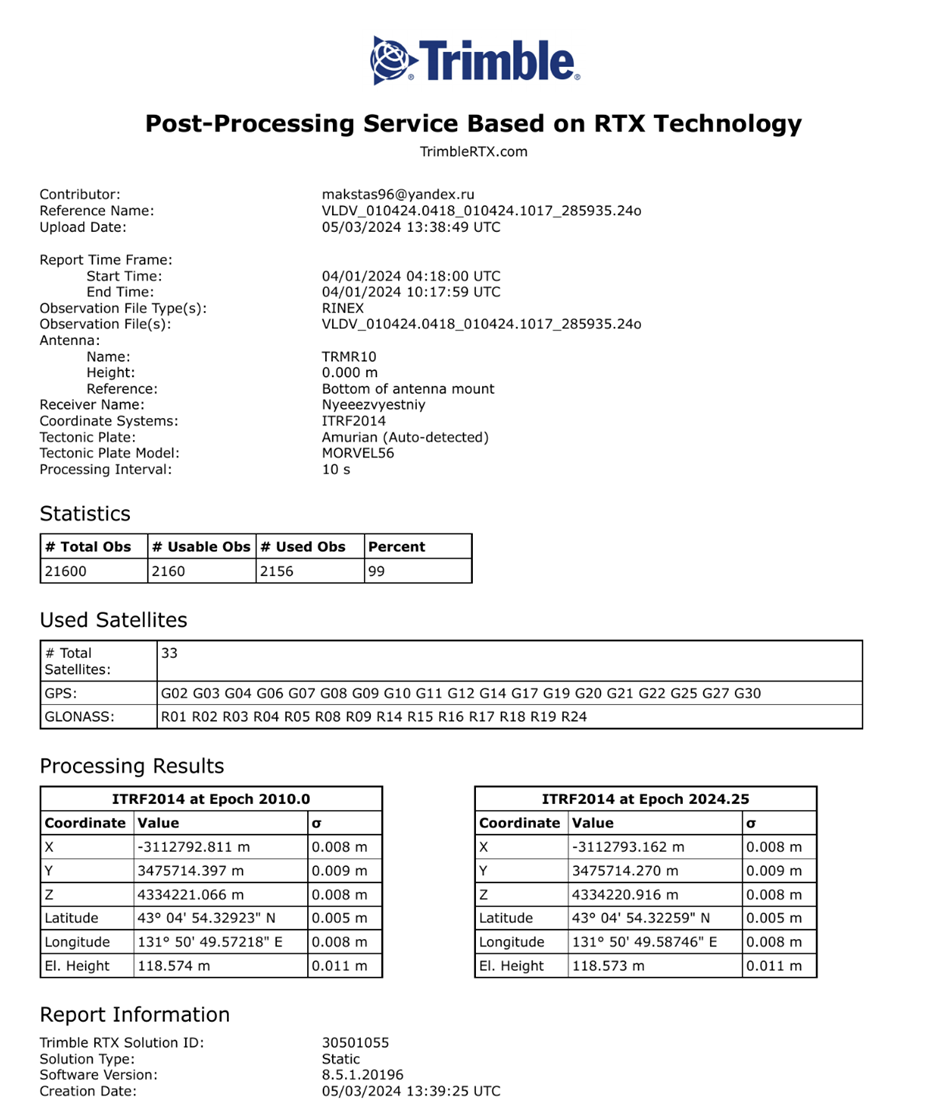
\includegraphics[width=\linewidth]{images/pic07}
	\caption{Пример отчета Trimble RTX}
	\label{fig:pic07}
\end{figure}

Как видно из рисунка \cref{fig:pic07} в отчете указывается вся интересующая информация: время начала и окончания измерения; количество используемых ГНСС и номер спутников; и координаты, приводимые на 2 эпохи в двух представлениях. В геодезической системе координат(BLH) и геоцентрической(XYZ). 

\subsection{Magic PPP (magic GNNS)}\label{subsec:ch2/sec1/sub2}

Magic PPP --- это глобальный сервис позиционирования, который позволяет пользователям GNSS определять своё положение или траекторию с сантиметровой точностью. 

Метод, используемый в magic PPP, не требует данных от непрерывных опорных станций (CORS), работающих в непосредственной близости от приемника. Идеальное решение для точной траектографии на больших расстояниях и/или в областях, отличных от покрытия CORS.

Данный сервис состоит из 4-х служб-составляющих. С более подробной информацией можно ознакомиться на официальном сайте \cite{src69}. 
 
 
\subsection{Canadian Spatial Reference System (CSRS-PPP)  }\label{subsec:ch2/sec1/sub3}
 
CSRS – Канадский сервис, предназначенный для обработки спутниковых данных по РРР-алгоритму.
 
Основные сведения о сервисе: 
 
\begin{list}{$ \checkmark $\\[6pt]} {\parsep = \parskip \itemsep=\parsep \topsep=0em}
	\item Бесплатный сервис. 
	\item Присутствует возможность обработки любых форматов сырых данных, собранных ГНСС-аппаратурой.
	\item Возможно, обрабатывать как статические, так и кинематические данные.
	\item Возможна загрузка как данных, собранных двухчастотным, так и одночастотным приемником.
\end{list}

В отличии от интернет-сервиса Trimble RTX у данного сервиса реализована обработка как статических, так и кинематических данных. 

Результаты обработки могут быть представлены как в системе координат ITRF, так и в локальной системе координат, применяемой на территории Северной Америки --- NAD-83. В \textbf{\underline{приложении F}} приведен отчет с данного интернет-сервиса.


\subsection{Automatic Precise Points Positioning Service (APPS)}\label{subsec:ch2/sec1/sub4}

APPS принимает файлы GPS-измерений и применяет самую передовую технологию GPS-позиционирования из Лаборатории реактивного движения NASA для оценки положения ваших GPS-приемников, независимо от того, находятся ли они в статике, в движении, на земле или в воздухе \cite{src80}.

Основные сведения о APPS:

\begin{list}{$ \checkmark $\\[6pt]} {\parsep = \parskip \itemsep=\parsep \topsep=0em}
	\item Бортовые эфемериды и поправки к часам в режиме реального времени GPS~JPL. 
	\item Уточненные и высокоточные (фиальные) эфемериды от JPL.
	\item Инернет-сервис и программное обеспечение  GIPSY-OASIS содержит один и тот же алгоритм.
	\item Поддерживает форматы данных: RINEX~2, RINEX~2.11 и фирменный формат данных GPSY~TDP.
\end{list}

\subsection{GNSS Analysis and Positioning Software (GAPS)}\label{subsec:ch2/sec1/sub5}

GAPS обеспечивает пользователям точное позиционирование с использованием одного спутникового приемника геодезического класса как в статическом, так и в кинематическом режиме. Благодаря использованию высокоточных эфемерид и поправок к часам, предоставляемых такими источниками, как Международная служба ГНСС (IGS) и Natural Resources Canada (NRCan), можно легко достичь точность на сантиметровом уровне в статическом режиме и позиционирования на дециметровом уровне в кинематическом режиме при достаточной продолжительности измерения.

\subsection{OPUS}\label{subsec:ch2/sec1/sub6}

Этот сервис предназначен для обработки спутниковых данных с использованием РРР-алгоритма. Он обеспечивает простой доступ к высокоточным координатам Национальной пространственной системы отсчета NSRS.  Для успешной реализации необходимо загрузить исходный файл, а обработанные координаты придут на указанную электронную почту.

OPUS требует минимального пользовательского ввода и обработка происходит с использованием программного обеспечения, которое вычисляет координаты для сетей NGS Continuous Operating Reference Station (далее «CORS»). 

У данного интернет-сервиса есть ряд требований, предъявляемых к сырым файлам:

\begin{list}{$ \checkmark $\\[6pt]} {\parsep = \parskip \itemsep=\parsep \topsep=0em}
	\item Данные должны быть собраны двухчастотным спутниковым приемником. 
	\item Возможно обрабатывать данные продолжительностью измерений начиная с 15 минут и заканчивая 48 часами.
	\item Файлы продолжительностью менее двух часов обязательно должны содержать не только P2, но и P1 или C1.
	\item Частота записи может быть 1,2,3,5,10,15,30 секунд.
	\item Необходимо правильно выбирать антенну и высоту антенны. Неправильно выбранный тип антенны может выдать ошибку измерений в плане до 1~см; по высоте до 80~см.
\end{list}

\subsection{SOPAC SCOUT (Scripps Coordinate Update Tool of Scripps Orbit and Permanent Array Centre)}\label{subsec:ch2/sec1/sub7}

В основе сервиса SOPAC SCOUT лежит тот же принцип, что и в остальных интернет-сервисах. Однако в сравнении с другими сервисами есть пару ключевых отличий:

\begin{list}{$ \checkmark $\\[6pt]} {\parsep = \parskip \itemsep=\parsep \topsep=0em}
	\item Можно обрабатывать не более 10 проектов одновременно. 
	\item Минимальная рекомендуемая продолжительность измерений --- 1 час.
\end{list}


\subsection{IBGE-PPP (Scripps Coordinate Update Tool of Scripps Orbit and Permanent Array Centre)}\label{subsec:ch2/sec1/sub8}

Интернет-сервис был разработан Бразильским институтом географии и статистики. При этом, как и в случае интернет-сервисов Trimble RTX и CRSR количество одновременно обрабатываемых RINEX-файлов не ограничено.


\subsection{IGN-PPP}\label{subsec:ch2/sec1/sub9}

Данный интернет-сервис был разработан Аргентинским научным сообществом. В основе данного сервиса лежит интернет сервис CSRS. В \textbf{\underline{приложении Б}} приведен отчёт данного интернет-сервиса.


\subsection{PPP AS A SERVICE}\label{subsec:ch2/sec1/su10}

Интернет-сервис был разработан российским научным сообществом. PAAS (PPP as a service) обеспечивает возможность быстрого расчёта. В \textbf{\underline{приложении В}} приведен отчёт данного интернет-сервиса.


\subsection{Сравнение интернет-сервисов между собой}\label{subsec:ch2/sec1/sub11}

С целью сравнения интернет-сервисов между собой была создана таблица \cref{tab:tab03}, в которой приведены основные сравнительные характеристики. Для компактной записи были использованы общепринятые обозначения R -- ГЛОНАСС, G -- GPS.


\noindent\begin{minipage}{\linewidth}
	\centering\vspace{5mm}
	\captionof{table}{Сравнение данных между собой}\label{tab:tab03}\resizebox{\linewidth}{!}{%
		\begin{tabular}{|c|c|c|c|c|c|c|c|}
			\hline
			\textbf{Критерий} & \textbf{RTX} & \textbf{CRSR} & \begin{tabular}[c]{@{}l@{}}\textbf{Magic}\\ \textbf{GNNS}\end{tabular} & \textbf{GAPS} & \textbf{APPS} & \textbf{OPUS} & \textbf{PAAS} \\
			\hline
			\textbf{Дискретность} & все & $\ge30$ сек. & все & все & все & все & все \\
			\hline
			\textbf{СК} & BLH, ITRF & \begin{tabular}[c]{@{}l@{}}BLH, NAD,\\ \ \ \ \ ITRF\end{tabular} & BLH, ITRF & BLH, ITRF & BLH, ITRF & \begin{tabular}[c]{@{}l@{}}BLH, ITRF,\\ \ \ \ \ \ \ UTM\end{tabular} &  \\
			\hline
			\textbf{$\mathbf{t_{min}}$ (мин)} & $10$ & $10$ & $10$ & $10$ & $10$ & $15$ &  \\
			\hline
			\textbf{$\mathbf{t_{max}}$ (ч)} & $24$ & $24$ & $24$ & $24$ & $24$ & $24$ &  \\
			\hline
			\textbf{$\mathbf{t_\text{обработки}}$ (мин)} & $2-3$ & $2-3$ & $4$ & $10-15$ & $5$ & $5$ & $3$ \\
			\hline
			\begin{tabular}[c]{@{}l@{}}\textbf{ \ \ \ ГНСС}\\\textbf{комбинации} \end{tabular} & R, G, C & R, G & R, G & R, G & R, G & R, G & R, G \\
			\hline
			\begin{tabular}[c]{@{}l@{}}\textbf{Количество}\\\textbf{ \ проектов}\end{tabular} & $\infty$ & $\infty$ & $\infty$ & $\infty$ & $\infty$ & $\infty$ &  \\
			\hline
		\end{tabular}
	}
\end{minipage}\vspace{5mm}


Из таблицы \cref{tab:tab03} видно, что с точки зрения времени, затрачиваемого на обработку измерений, быстрее происходит предоставление результатов в случае использования RTX и CRSR. Однако у CRSR обработка данных выполняется только при периодичности записи 30 секунд и реже. Конечно, можно использовать и более высокую частоту, но в таком случае данные будут прорежены, что может привести к существенному снижению точности получаемого решения. Также можно заключить, что интернет-сервис SOPAC SCOUT выполняет работу медленнее прочих.



\section{Обзор современных программных обеспечений для обработки РРР}\label{sec:ch2/sec2}

\subsection{Bernese} \label{subsec:ch2/sec2/sub1}

Программное обучение Bernese было разработано в астрономическом институте Бернского университета для постобработки наблюдений GNSS в научных исследованиях \cite{src47}. Это программное обеспечение используется Европейским орбитальным центром (Code) для поддержки международных (IGS) и европейских (EUREF/EPN) глобальных спутниковых навигационных сетей. 

В программном обеспечении можно обрабатывать как статические, так и кинематические наблюдения. Помимо этого, используя программное обеспечение Bernese существует возможность обрабатывать данные в результате высокоточного позиционирования (РРР). Благодаря встроенным моделям существует возможность учитывать движение литосферных плит, грунтов, а также приливы и отливы. К тому же постоянно поддерживается учет зенитной тропосферной задержки и градиента, параметров ориентации Земли и глобальных ионосферных моделей \cite{src51,src52}.

\subsection{GIPSY-OASIS} \label{subsec:ch2/sec2/sub2}

Лаборатория реактивного движения Национального управления по аэронавтике и исследованию космического пространства (НАСА) в Пасадене, штат Калифорния, обеспечивает поддержку пользователей GIPSY-OASIS (GOA II) --- автоматизированного, быстрого, сверхточного программного комплекса для обработки высокоточных данных GPS со строгим контролем качества данных.

\subsection{Waypoint Grafnet} \label{subsec:ch2/sec2/sub3}

Программное обеспечение для постобработки Graphnet --- это мощный программный комплекс, для обеспечения наилучшей статической или кинематической точности ГНСС с использованием всех доступных данных ГНСС. Поддержка форматов данных для большинства одно- и многочастотных коммерческих приемников означает, что Graphnav, скорее всего, будет работать с существующим оборудованием \cite{src67}.

\subsection{RTKLIB} \label{subsec:ch2/sec2/sub4}

RTKLIB --- набор библиотек с открытым кодом. Данное программное обеспечение предназначено для обработки как статических, так и кинематических данных \cite{src72}. Среди преимуществ данного программного обеспечения стоит выделить возможность обработки данных только ГЛОНАСС, что ни в одном другом программном обеспечении или интернет-сервисе не реализовано.  

\subsection{КРЕДО ГНСС} \label{subsec:ch2/sec2/sub5}

В программном обеспечении КРЕДО ГНСС присутствует возможность обработки спутниковых данных не только по стандартным алгоритмам, но и при использовании методов высокоточных координатных определений. Данная возможность появилась с выходом версии 2.0.

\subsection{Trimble Business Centre}\label{subsec:ch2/sec2/sub6}

В современных версиях программного обеспечения Trimble Bisiness Centre (далее «TBC») присутствует возможность не только обработки спутниковых данных, но также данных с применением наземных методов, фотограмметрии и результатов лазерного сканирования. Кроме того в программном обеспечении реализована возможность обработки данных и по РРР-алгоритму \cite{src65,src67}.

\subsection{TropoGNSS}\label{subsec:ch2/sec2/sub7}

TropoGNSS --- программный продукт для мониторинга параметров атмосферы и движений земной коры, рассчитываемых по измерениям сигналов Глобальных Навигационных Спутниковых Систем (ГНСС). Данное приложение разработано в Казанском федеральном университете и является одним из немногих примеров российских научных программных продуктов в этой сфере. В TropoGNSS реализован абсолютный метод обработки данных ГНСС, называемый технологией PPP (Precise Point Positioning). Эта технология предполагает получение высокоточных результатов по данным одиночной станции. Применяемый в программе алгоритм основан на сравнении длин геометрического и фазового пути радиоволн от спутников ГНСС до наземного приемника. Уравнивание измерений производится с помощью фильтра Калмана. В настоящее время приложение поддерживает обработку данных американской системы GPS, российской системы ГЛОНАСС и европейской системы Galileo.

\subsection{ПроГеоСеть}\label{subsec:ch2/sec2/sub8}

ПроГеоСеть современный программный продукт, представленный разработчиками в январе 2024 года. По заявлению разработчика (НИИ Микроэлектронной аппаратуры Прогресс) программное обеспечение является частью геодезического комплекса ПРОГЕО. По заявлению разработчиков данное программное обеспечение предназначено для: позиционирования и навигации статических и подвижных объектов на основе данных спутниковых систем GPS, ГЛОНАСС, Galileo, Beidou, QZSS, IRNSS методами RTK, RTPK, PPP и классической постобработкой \cite{src36}.

Помимо выше перечисленного, в настоящее время, по заявлению производителей, программное обеспечение происходит процедуру сертификации и в геодезическом производстве \textbf{\textit{будет использоваться с середины 2024 года}}.


\section{Исследование точности определения координат, при использовании современных способов обработки данных по РРР-алгоритму}\label{sec:ch2/sec3}

Полевые экспериментальные работы выполнялись с 21.01.2022 по 14.02.2022 в общей сложности --- 12 дней по 3-5 часов ежедневно на крыше седьмого корпуса РУТ(МИИТ) с использованием двухчастотного спутникового приемника Trimble R10. На рисунке \cref{fig:pic01} представлен описываемый пункт (MIIT).

\begin{figure}[h]
	\centering
	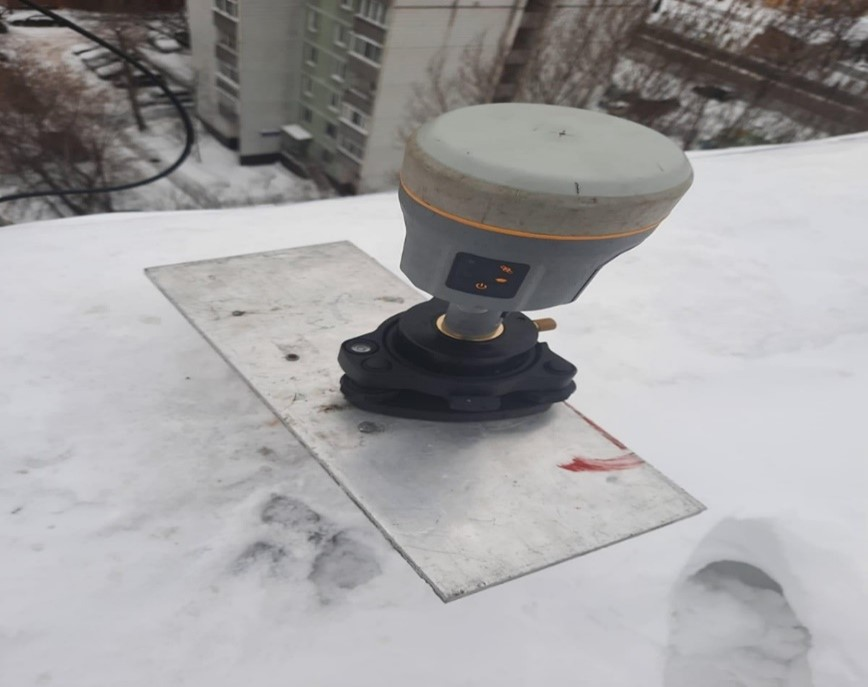
\includegraphics[width=0.7\linewidth]{images/pic08}
	\caption{Спутниковый приемник на крыше}
	\label{fig:pic08}
\end{figure}

Периодичность записи измерений составляла 10 секунд.  Среднее время проведения экспериментальных работ с 12:00 до 15:00. После проведения съёмочных работ сырые файлы преобразовывались в формат RINEX версии 2.11 с использованием программного обеспечения Trimble Convert to RINEX \cite{src84}. 

Для исследования точности обработки данных по РРР-алгоритму были поставлены следующие цели:

\begin{enumerate}
	\item Выявить влияние продолжительности измерений на данные, получаемые при обработке по РРР-алгоритму. 
	\item Выявить влияние количества принимаемых спутников и оценить влияние pdop фактора на получаемые результаты.
	\item Проанализировать точность при использовании ГНСС в различных комбинациях (только ГЛОНАСС; только GPS; совместно ГЛОНАСС и GPS).
	\item Рассмотреть получаемую точность при обработке многократных спутниковых измерений.
	\item Рассмотреть влияние частоты записи \textbf{на получаемые приращения координат}.
	\item Произвести сравнение между реализациями с использованием программных обеспечений и интернет-сервисов.
\end{enumerate}

Этапы проведения работ и полученные результаты приведены в пунктах \cref{subsec:ch2/sec3/sub1}, \cref{subsec:ch2/sec3/sub2}, \cref{subsec:ch2/sec3/sub3}, \cref{subsec:ch2/sec3/sub4}, \cref{subsec:ch2/sec3/sub5}.




\subsection[Влияние многократных измерений]{Исследование точности при многократных спутниковых измерениях}\label{subsec:ch2/sec3/sub1}

Для исследования координат, определяемых по РРР-алгоритму \textit{с точки зрения многократных измерений}, было выполнено следующее:
%были подготовлены RINEX-файлы, содержащие одно-, двух- и трёхчасовые интервалы измерений.
\begin{enumerate}
	\item Были подготовлены RINEX-файлы, содержащие трёхчасовые интервалы измерений. 
	\item Впоследствии RINEX-файлы были преобразованы в наборы данных, содержащие одно-, двух- и трёхчасовые интервалы.
\end{enumerate}

\subsubsection{Обработка с использованием интернет-сервиса Trimble RTX }\label{subsec:ch2/sec3/sub1/sub1}

Обработка данных РРР-алгоритмом по RTX обработке, производится на сайте Trimble-RTX \cite{src44}. Обработка выполняется автоматически после загрузки RINEX-файла. По её завершении можно скачать результаты.

Этот процесс повторяется последовательно ко всем RINEX-файлам. Ниже, в таблице \cref{tab:tab04}, приведены координаты пункта (MIIT), полученные из \textit{одночасовых} измерений, выполнявшихся в течение двенадцати дней.

\begin{table} [h!]
	\centering\small
	\captionof{table}{Координаты пункта MIIT. Сервис Trimble RTX, $T_{\text{изм.}}=1$ час}\label{tab:tab04}{%
		\begin{tabular}{|c|c|c|c|c|}
			\hline
			\textbf{№} & \textbf{Дата} & \textbf{X, м} & \textbf{Y, м} & \textbf{Z, м} \\
			\hline
			\textbf{ $\mathbf{1}$} & $21.01.2022$ & $2847750,924$ & $2193184,486$ & $5251441,725$ \\
			\hline
			\textbf{ $\mathbf{2}$} & $26.01.2022$ & $2847750,932$ & $2193184,486$ & $5251441,735$ \\
			\hline
			\textbf{ $\mathbf{3}$} & $27.01.2022$ & $2847750,927$ & $2193184,487$ & $5251441,733$ \\
			\hline
			\textbf{ $\mathbf{4}$} & $28.01.2022$ & $2847750,934$ & $2193184,486$ & $5251441,737$ \\
			\hline
			\textbf{ $\mathbf{5}$} & $31.01.2022$ & $2847750,945$ & $2193184,494$ & $5251441,735$ \\
			\hline
			\textbf{ $\mathbf{6}$} & $01.02.2022$ & $2847750,927$ & $2193184,475$ & $5251441,703$ \\
			\hline
			\textbf{ $\mathbf{7}$} & $02.02.2022$ & $2847750,931$ & $2193184,483$ & $5251441,730$ \\
			\hline
			\textbf{ $\mathbf{8}$} & $03.02.2022$ & $2847750,933$ & $2193184,483$ & $5251441,725$ \\
			\hline
			\textbf{ $\mathbf{9}$} & $04.02.2022$ & $2847750,933$ & $2193184,481$ & $5251441,723$ \\
			\hline
			\textbf{$\mathbf{10}$} & $09.02.2022$ & $2847750,930$ & $2193184,488$ & $5251441,733$ \\
			\hline
			\textbf{$\mathbf{11}$} & $10.02.2022$ & $2847750,934$ & $2193184,491$ & $5251441,740$ \\
			\hline
			\textbf{$\mathbf{12}$} & $14.02.2022$ & $2847750,946$ & $2193184,496$ & $5251441,736$ \\
			\hline
		\end{tabular}
	}
\end{table}

В таблице \cref{tab:tab05} приведены координаты пункта (MIIT), полученные из \textit{двухчасовых} измерений, выполнявшихся в течение двенадцати дней.

\begin{table} [htbp]
	\centering\small
	\captionof{table}{Координаты пункта MIIT. Сервис Trimble RTX, $T_{\text{изм.}}=2$ часа}\label{tab:tab05}{%
		\begin{tabular}{|c|c|c|c|c|}
			\hline
			\textbf{№} & \textbf{Дата} & \textbf{X, м} & \textbf{Y, м} & \textbf{Z, м} \\
			\hline
			\textbf{ $\mathbf{1}$} & $21.01.2022$ & $2847750,925$ & $2193184,483$ & $5251441,713$ \\
			\hline
			\textbf{ $\mathbf{2}$} & $26.01.2022$ & $2847750,928$ & $2193184,487$ & $5251441,722$ \\
			\hline
			\textbf{ $\mathbf{3}$} & $27.01.2022$ & $2847750,930$ & $2193184,487$ & $5251441,723$ \\
			\hline
			\textbf{ $\mathbf{4}$} & $28.01.2022$ & $2847750,937$ & $2193184,491$ & $5251441,733$ \\
			\hline
			\textbf{ $\mathbf{5}$} & $31.01.2022$ & $2847750,941$ & $2193184,496$ & $5251441,737$ \\
			\hline
			\textbf{ $\mathbf{6}$} & $01.02.2022$ & $2847750,932$ & $2193184,488$ & $5251441,722$ \\
			\hline
			\textbf{ $\mathbf{7}$} & $02.02.2022$ & $2847750,937$ & $2193184,492$ & $5251441,736$ \\
			\hline
			\textbf{ $\mathbf{8}$} & $03.02.2022$ & $2847750,934$ & $2193184,492$ & $5251441,728$ \\
			\hline
			\textbf{ $\mathbf{9}$} & $04.02.2022$ & $2847750,938$ & $2193184,490$ & $5251441,734$ \\
			\hline
			\textbf{$\mathbf{10}$} & $09.02.2022$ & $2847750,933$ & $2193184,491$ & $5251441,729$ \\
			\hline
			\textbf{$\mathbf{11}$} & $10.02.2022$ & $2847750,932$ & $2193184,487$ & $5251441,725$ \\
			\hline
			\textbf{$\mathbf{12}$} & $14.02.2022$ & $2847750,939$ & $2193184,490$ & $5251441,728$ \\
			\hline
		\end{tabular}
	}
\end{table}

В таблице \cref{tab:tab06} приведены координаты пункта (MIIT), полученные из \textit{трёхчасовых} измерений выполнявшихся в течение двенадцати дней.

\begin{table} [htbp]
	\centering\small
	\captionof{table}{Координаты пункта MIIT. Сервис Trimble RTX, $T_{\text{изм.}}=3$ часа}\label{tab:tab06}{%
		\begin{tabular}{|c|c|c|c|c|}
			\hline
			\textbf{№} & \textbf{Дата} & \textbf{X, м} & \textbf{Y, м} & \textbf{Z, м} \\
			\hline
			\textbf{ $\mathbf{1}$} & $21.01.2022$ & $2847750,927$ & $2193184,485$ & $5251441,714$ \\
			\hline
			\textbf{ $\mathbf{2}$} & $26.01.2022$ & $2847750,932$ & $2193184,489$ & $5251441,724$ \\
			\hline
			\textbf{ $\mathbf{3}$} & $27.01.2022$ & $2847750,933$ & $2193184,488$ & $5251441,724$ \\
			\hline
			\textbf{ $\mathbf{4}$} & $28.01.2022$ & $2847750,939$ & $2193184,493$ & $5251441,734$ \\
			\hline
			\textbf{ $\mathbf{5}$} & $31.01.2022$ & $2847750,943$ & $2193184,497$ & $5251441,736$ \\
			\hline
			\textbf{ $\mathbf{6}$} & $01.02.2022$ & $2847750,933$ & $2193184,488$ & $5251441,723$ \\
			\hline
			\textbf{ $\mathbf{7}$} & $02.02.2022$ & $2847750,937$ & $2193184,491$ & $5251441,732$ \\
			\hline
			\textbf{ $\mathbf{8}$} & $03.02.2022$ & $2847750,933$ & $2193184,489$ & $5251441,721$ \\
			\hline
			\textbf{ $\mathbf{9}$} & $04.02.2022$ & $2847750,940$ & $2193184,489$ & $5251441,727$ \\
			\hline
			\textbf{$\mathbf{10}$} & $09.02.2022$ & $2847750,931$ & $2193184,486$ & $5251441,721$ \\
			\hline
			\textbf{$\mathbf{11}$} & $10.02.2022$ & $2847750,932$ & $2193184,485$ & $5251441,721$ \\
			\hline
			\textbf{$\mathbf{12}$} & $14.02.2022$ & $2847750,938$ & $2193184,489$ & $5251441,723$ \\
			\hline
		\end{tabular}
	}
\end{table}

В дальнейшем были найдены разности приращений координат между вычисленными и усредненными координатами, сведёнными в таблицу \cref{tab:tab07}. 
Значения усредненных координат: 
$$
	\left\{
	\begin{matrix}
		\overline{X} = 2847750,943 \pm 000,000 \text{ м}, \\
		\overline{Y} = 2193184,497 \pm 000,000 \text{ м}, \\
		\overline{Z} = 5251441,736 \pm 000,000 \text{ м.}
	\end{matrix}
	\right.
$$

\begin{table} [htbp]
	\centering\small
	\captionof{table}{Разности координат. Сервис Trimble RTX}\label{tab:tab07}{%
		\begin{tabular}{|c|rrr|rrr|rrr|}
			\hline
			\multirow{2}{*}{\textbf{№}} & 
			\multicolumn{3}{c|}{\textbf{1 час}}                                                                             & \multicolumn{3}{c|}{\textbf{2 часа}}                                                                            & \multicolumn{3}{c|}{\textbf{3 часа}}                                                                            \\ \cline{2-10} 
			& \multicolumn{1}{l|}{\textbf{σX, м}} & \multicolumn{1}{l|}{\textbf{σY, м}} & \multicolumn{1}{l|}{\textbf{σZ, м}} & \multicolumn{1}{l|}{\textbf{σX, м}} & \multicolumn{1}{l|}{\textbf{σY, м}} & \multicolumn{1}{l|}{\textbf{σZ, м}} & \multicolumn{1}{l|}{\textbf{σX, м}} & \multicolumn{1}{l|}{\textbf{σY, м}} & \multicolumn{1}{l|}{\textbf{σZ, м}} \\ \hline
			\textbf{1}                  & 
			\multicolumn{1}{r|}{$ 0,019$}       & \multicolumn{1}{r|}{$-0,011$}       & $-0,011$                            & \multicolumn{1}{r|}{$ 0,018$}       & \multicolumn{1}{r|}{$-0,014$}       & $-0,023$                            & \multicolumn{1}{r|}{$ 0,016$}       & \multicolumn{1}{r|}{$-0,012$}       & $-0,022$                            \\ \hline
			\textbf{2}                  & 
			\multicolumn{1}{r|}{$-0,011$}       & \multicolumn{1}{r|}{$-0,011$}       & $-0,001$                            & \multicolumn{1}{r|}{$-0,015$}       & \multicolumn{1}{r|}{$-0,010$}       & $-0,014$                            & \multicolumn{1}{r|}{$-0,011$}       & \multicolumn{1}{r|}{$-0,008$}       & $-0,012$                            \\ \hline
			\textbf{3}                  & 
			\multicolumn{1}{r|}{$-0,016$}       & \multicolumn{1}{r|}{$-0,010$}       & $-0,003$                            & \multicolumn{1}{r|}{$-0,013$}       & \multicolumn{1}{r|}{$-0,010$}       & $-0,013$                            & \multicolumn{1}{r|}{$-0,010$}       & \multicolumn{1}{r|}{$-0,009$}       & $-0,012$                            \\ \hline
			\textbf{4}                  & 
			\multicolumn{1}{r|}{$-0,019$}        & \multicolumn{1}{r|}{$-0,011$}       & $-0,011$                            & \multicolumn{1}{r|}{$-0,018$}        & \multicolumn{1}{r|}{$-0,014$}       & $-0,023$                            & \multicolumn{1}{r|}{$-0,016$}        & \multicolumn{1}{r|}{$-0,012$}       & $-0,022$                            \\ \hline
			\textbf{5}                  & 
			\multicolumn{1}{r|}{$-0,011$}        & \multicolumn{1}{r|}{$-0,011$}       & $-0,001$                            & \multicolumn{1}{r|}{$-0,015$}        & \multicolumn{1}{r|}{$-0,010$}       & $-0,014$                            & \multicolumn{1}{r|}{$-0,011$}        & \multicolumn{1}{r|}{$-0,008$}       & $-0,012$                            \\ \hline
			\textbf{6}                  & 
			\multicolumn{1}{r|}{$-0,016$}        & \multicolumn{1}{r|}{$-0,010$}       & $-0,003$                            & \multicolumn{1}{r|}{$-0,013$}        & \multicolumn{1}{r|}{$-0,010$}       & $-0,013$                            & \multicolumn{1}{r|}{$-0,010$}        & \multicolumn{1}{r|}{$-0,009$}       & $-0,012$                            \\ \hline
			\textbf{7}                  & 
			\multicolumn{1}{r|}{$ 0,012$}        & \multicolumn{1}{r|}{$-0,014$}       & $-0,006$                            & \multicolumn{1}{r|}{$ 0,006$}        & \multicolumn{1}{r|}{$-0,005$}       & $ 0,000$                            & \multicolumn{1}{r|}{$ 0,006$}        & \multicolumn{1}{r|}{$-0,006$}       & $-0,004$                            \\ \hline
			\textbf{8}                  & 
			\multicolumn{1}{r|}{$-0,010$}        & \multicolumn{1}{r|}{$-0,014$}       & $-0,011$                            & \multicolumn{1}{r|}{$-0,009$}        & \multicolumn{1}{r|}{$-0,005$}       & $-0,008$                            & \multicolumn{1}{r|}{$-0,010$}        & \multicolumn{1}{r|}{$-0,008$}       & $-0,015$                            \\ \hline
			\textbf{9}                  & 
			\multicolumn{1}{r|}{$-0,010$}        & \multicolumn{1}{r|}{$-0,016$}       & $-0,013$                            & \multicolumn{1}{r|}{$-0,005$}        & \multicolumn{1}{r|}{$-0,007$}       & $-0,002$                            & \multicolumn{1}{r|}{$-0,003$}        & \multicolumn{1}{r|}{$-0,008$}       & $-0,009$                            \\ \hline
			\textbf{10}                 & 
			\multicolumn{1}{r|}{$-0,013$}        & \multicolumn{1}{r|}{$-0,009$}       & $-0,003$                            & \multicolumn{1}{r|}{$-0,010$}        & \multicolumn{1}{r|}{$-0,006$}       & $-0,007$                            & \multicolumn{1}{r|}{$-0,012$}        & \multicolumn{1}{r|}{$-0,011$}       & $-0,015$                            \\ \hline
			\textbf{11}                 & 
			\multicolumn{1}{r|}{$-0,009$}        & \multicolumn{1}{r|}{$-0,006$}       & $ 0,004$                            & \multicolumn{1}{r|}{$-0,011$}        & \multicolumn{1}{r|}{$-0,010$}       & $-0,011$                            & \multicolumn{1}{r|}{$-0,011$}        & \multicolumn{1}{r|}{$-0,012$}       & $-0,015$                            \\ \hline
			\textbf{12}                 & 
			\multicolumn{1}{r|}{$ 0,003$}        & \multicolumn{1}{r|}{$-0,001$}       & $ 0,000$                            & \multicolumn{1}{r|}{$-0,004$}        & \multicolumn{1}{r|}{$-0,007$}       & $-0,008$                            & \multicolumn{1}{r|}{$-0,005$}        & \multicolumn{1}{r|}{$-0,008$}       & $-0,013$                            \\ \hline
		\end{tabular}
	}
\end{table}


В таблице \cref{tab:tab08} приводятся средние, а также минимальные и максимальные значения разностей координат.

\begin{table} [htbp]
	\centering\small
	\captionof{table}{Обобщённые разности координат. Сервис Trimble RTX}\label{tab:tab08}{%\resizebox{\linewidth}{!}{%
		\begin{tabular}{|c|rrr|rrr|rrr|}
			\hline
			\multirow{2}{*}{\textbf{ }} & 
			\multicolumn{3}{c|}{\textbf{1 час}}  & \multicolumn{3}{c|}{\textbf{2 часа}}  & \multicolumn{3}{c|}{\textbf{3 часа}}  \\ \cline{2-10} & 
			\multicolumn{1}{l|}{\textbf{σX, м}} & \multicolumn{1}{l|}{\textbf{σY, м}} & \multicolumn{1}{l|}{\textbf{σZ, м}} & \multicolumn{1}{l|}{\textbf{σX, м}} & \multicolumn{1}{l|}{\textbf{σY, м}} & \multicolumn{1}{l|}{\textbf{σZ, м}} & \multicolumn{1}{l|}{\textbf{σX, м}} & \multicolumn{1}{l|}{\textbf{σY, м}} & \multicolumn{1}{l|}{\textbf{σZ, м}} \\ \hline
			\textbf{мин.}                       & \multicolumn{1}{r|}{$-0,019$}       & \multicolumn{1}{r|}{$-0,022$}         & $-0,033$                            & \multicolumn{1}{r|}{$-0,018$}       & \multicolumn{1}{r|}{$-0,014$}         & $-0,023$                            & \multicolumn{1}{r|}{$-0,016$}       & \multicolumn{1}{r|}{$-0,012$}         & $-0,022$                              \\ \hline
			\textbf{макс.}                      & \multicolumn{1}{r|}{$0,003$}        & \multicolumn{1}{r|}{$-0,001$}         & $0,004$                             & \multicolumn{1}{r|}{$-0,002$}       & \multicolumn{1}{r|}{$-0,001$}         & $0,001$                             & \multicolumn{1}{r|}{$0,000$}        & \multicolumn{1}{r|}{$0,000$}          & $0,000$                              \\ \hline
			\textbf{среднее}                    & \multicolumn{1}{r|}{$-0,010$}       & \multicolumn{1}{r|}{$-0,011$}         & $-0,006$                            & \multicolumn{1}{r|}{$-0,009$}       & \multicolumn{1}{r|}{$-0,007$}         & $-0,008$                            & \multicolumn{1}{r|}{$-0,008$}       & \multicolumn{1}{r|}{$-0,008$}         & $-0,011$                              \\ \hline
		\end{tabular}
	}
\end{table}

Анализируя таблицу \cref{tab:tab08} можно заметить, что в среднем величины отклонений координат содержат одинаковую ошибку при 12-дневыных измерениях.




\subsubsection{Обработка с использованием интернет-сервиса CSRS }\label{subsec:ch2/sec3/sub1/sub2}


Обработка происходила интернет-сервисом CSRS. Был использован тот же набор RINEX-файлов данных. Этапы обработки те же самые. Результаты приведены в таблице \cref{tab:tab09}.


\begin{table} [htbp]
	\centering\small
	\captionof{table}{Разности координат. Сервис CSRS}\label{tab:tab09}{%
		\begin{tabular}{|c|rrr|rrr|rrr|}
			\hline
			\multirow{2}{*}{\textbf{№}} & 
			\multicolumn{3}{c|}{\textbf{1 час}}                                                                             & \multicolumn{3}{c|}{\textbf{2 часа}}                                                                            & \multicolumn{3}{c|}{\textbf{3 часа}}                                                                            \\ \cline{2-10} 
			& \multicolumn{1}{l|}{\textbf{σX, м}} & \multicolumn{1}{l|}{\textbf{σY, м}} & \multicolumn{1}{l|}{\textbf{σZ, м}} & \multicolumn{1}{l|}{\textbf{σX, м}} & \multicolumn{1}{l|}{\textbf{σY, м}} & \multicolumn{1}{l|}{\textbf{σZ, м}} & \multicolumn{1}{l|}{\textbf{σX, м}} & \multicolumn{1}{l|}{\textbf{σY, м}} & \multicolumn{1}{l|}{\textbf{σZ, м}} \\ \hline
			\textbf{1}                  & 
			\multicolumn{1}{r|}{$ 0,019$}       & \multicolumn{1}{r|}{$-0,011$}       & $-0,011$                            & \multicolumn{1}{r|}{$ 0,018$}       & \multicolumn{1}{r|}{$-0,014$}       & $-0,023$                            & \multicolumn{1}{r|}{$ 0,016$}       & \multicolumn{1}{r|}{$-0,012$}       & $-0,022$                            \\ \hline
			\textbf{2}                  & 
			\multicolumn{1}{r|}{$-0,011$}       & \multicolumn{1}{r|}{$-0,011$}       & $-0,001$                            & \multicolumn{1}{r|}{$-0,015$}       & \multicolumn{1}{r|}{$-0,010$}       & $-0,014$                            & \multicolumn{1}{r|}{$-0,011$}       & \multicolumn{1}{r|}{$-0,008$}       & $-0,012$                            \\ \hline
			\textbf{3}                  & 
			\multicolumn{1}{r|}{$-0,016$}       & \multicolumn{1}{r|}{$-0,010$}       & $-0,003$                            & \multicolumn{1}{r|}{$-0,013$}       & \multicolumn{1}{r|}{$-0,010$}       & $-0,013$                            & \multicolumn{1}{r|}{$-0,010$}       & \multicolumn{1}{r|}{$-0,009$}       & $-0,012$                            \\ \hline
			\textbf{4}                  & 
			\multicolumn{1}{r|}{$-0,019$}       & \multicolumn{1}{r|}{$-0,011$}       & $-0,011$                            & \multicolumn{1}{r|}{$-0,018$}       & \multicolumn{1}{r|}{$-0,014$}       & $-0,023$                            & \multicolumn{1}{r|}{$-0,016$}       & \multicolumn{1}{r|}{$-0,012$}       & $-0,022$                            \\ \hline
			\textbf{5}                  & 
			\multicolumn{1}{r|}{$-0,011$}       & \multicolumn{1}{r|}{$-0,011$}       & $-0,001$                            & \multicolumn{1}{r|}{$-0,015$}       & \multicolumn{1}{r|}{$-0,010$}       & $-0,014$                            & \multicolumn{1}{r|}{$-0,011$}       & \multicolumn{1}{r|}{$-0,008$}       & $-0,012$                            \\ \hline
			\textbf{6}                  & 
			\multicolumn{1}{r|}{$-0,016$}       & \multicolumn{1}{r|}{$-0,010$}       & $-0,003$                            & \multicolumn{1}{r|}{$-0,013$}       & \multicolumn{1}{r|}{$-0,010$}       & $-0,013$                            & \multicolumn{1}{r|}{$-0,010$}       & \multicolumn{1}{r|}{$-0,009$}       & $-0,012$                            \\ \hline
			\textbf{7}                  & 
			\multicolumn{1}{r|}{$ 0,012$}       & \multicolumn{1}{r|}{$-0,014$}       & $-0,006$                            & \multicolumn{1}{r|}{$ 0,006$}       & \multicolumn{1}{r|}{$-0,005$}       & $ 0,000$                            & \multicolumn{1}{r|}{$ 0,006$}       & \multicolumn{1}{r|}{$-0,006$}       & $-0,004$                            \\ \hline
			\textbf{8}                  & 
			\multicolumn{1}{r|}{$-0,010$}       & \multicolumn{1}{r|}{$-0,014$}       & $-0,011$                            & \multicolumn{1}{r|}{$-0,009$}       & \multicolumn{1}{r|}{$-0,005$}       & $-0,008$                            & \multicolumn{1}{r|}{$-0,010$}       & \multicolumn{1}{r|}{$-0,008$}       & $-0,015$                            \\ \hline
			\textbf{9}                  & 
			\multicolumn{1}{r|}{$-0,010$}       & \multicolumn{1}{r|}{$-0,016$}       & $-0,013$                            & \multicolumn{1}{r|}{$-0,005$}       & \multicolumn{1}{r|}{$-0,007$}       & $-0,002$                            & \multicolumn{1}{r|}{$-0,003$}       & \multicolumn{1}{r|}{$-0,008$}       & $-0,009$                            \\ \hline
			\textbf{10}                 & 
			\multicolumn{1}{r|}{$-0,013$}       & \multicolumn{1}{r|}{$-0,009$}       & $-0,003$                            & \multicolumn{1}{r|}{$-0,010$}       & \multicolumn{1}{r|}{$-0,006$}       & $-0,007$                            & \multicolumn{1}{r|}{$-0,012$}       & \multicolumn{1}{r|}{$-0,011$}       & $-0,015$                            \\ \hline
			\textbf{11}                 & 
			\multicolumn{1}{r|}{$-0,009$}       & \multicolumn{1}{r|}{$-0,006$}       & $ 0,004$                            & \multicolumn{1}{r|}{$-0,011$}       & \multicolumn{1}{r|}{$-0,010$}       & $-0,011$                            & \multicolumn{1}{r|}{$-0,011$}       & \multicolumn{1}{r|}{$-0,012$}       & $-0,015$                            \\ \hline
			\textbf{12}                 & 
			\multicolumn{1}{r|}{$ 0,003$}       & \multicolumn{1}{r|}{$-0,001$}       & $ 0,000$                            & \multicolumn{1}{r|}{$-0,004$}       & \multicolumn{1}{r|}{$-0,007$}       & $-0,008$                            & \multicolumn{1}{r|}{$-0,005$}       & \multicolumn{1}{r|}{$-0,008$}       & $-0,013$                            \\ \hline
		\end{tabular}
	}
\end{table}

Основываясь на таблице \cref{tab:tab09} была создана таблица \cref{tab:tab10}, в которой указываются максимальные, минимальные и средние разности координат.


\begin{table} [htbp]
	\centering\small
	\captionof{table}{Обобщённые разности координат. Сервис CSRS}\label{tab:tab10}{%\resizebox{\linewidth}{!}{%
		\begin{tabular}{|c|rrr|rrr|rrr|}
			\hline
			\multirow{2}{*}{\textbf{ }} & 
			\multicolumn{3}{c|}{\textbf{1 час}}  & \multicolumn{3}{c|}{\textbf{2 часа}}  & \multicolumn{3}{c|}{\textbf{3 часа}}  \\ \cline{2-10} & 
			\multicolumn{1}{l|}{\textbf{σX, м}} & \multicolumn{1}{l|}{\textbf{σY, м}} & \multicolumn{1}{l|}{\textbf{σZ, м}} & \multicolumn{1}{l|}{\textbf{σX, м}} & \multicolumn{1}{l|}{\textbf{σY, м}} & \multicolumn{1}{l|}{\textbf{σZ, м}} & \multicolumn{1}{l|}{\textbf{σX, м}} & \multicolumn{1}{l|}{\textbf{σY, м}} & \multicolumn{1}{l|}{\textbf{σZ, м}} \\ \hline
			\textbf{мин.}                    & 
			\multicolumn{1}{r|}{$-0,022$}       & \multicolumn{1}{r|}{$-0,014$}         & $-0,027$                            & \multicolumn{1}{r|}{$-0,026$}       & \multicolumn{1}{r|}{$-0,006$}         & $-0,022$                            & \multicolumn{1}{r|}{$-0,025$}       & \multicolumn{1}{r|}{$-0,011$}         & $-0,027$                            \\ \hline
			\textbf{макс.}                   & 
			\multicolumn{1}{r|}{$-0,002$}       & \multicolumn{1}{r|}{$ 0,015$}         & $ 0,018$                            & \multicolumn{1}{r|}{$-0,005$}       & \multicolumn{1}{r|}{$ 0,008$}         & $ 0,010$                            & \multicolumn{1}{r|}{$-0,008$}       & \multicolumn{1}{r|}{$ 0,003$}         & $ 0,003$                            \\ \hline
			\textbf{среднее}                    & 
			\multicolumn{1}{r|}{$-0,010$}       & \multicolumn{1}{r|}{$-0,002$}         & $-0,003$                            & \multicolumn{1}{r|}{$-0,015$}       & \multicolumn{1}{r|}{$ 0,000$}         & $-0,005$                            & \multicolumn{1}{r|}{$-0,017$}       & \multicolumn{1}{r|}{$-0,005$}         & $-0,013$                            \\ \hline
		\end{tabular}
	}
\end{table}



\subsubsection{Обработка с использованием интернет-сервиса GAPS }\label{subsec:ch2/sec3/sub1/sub3}

Последовательность обработки аналогична используемым в остальных интернет-сервисах. В таблице \cref{tab:tab11} приведены разности координат для всех двенадцати сеансов измерений.


\begin{table} [htbp]
	\centering\small
	\captionof{table}{Разности координат. Сервис GAPS}\label{tab:tab11}{%
		\begin{tabular}{|c|rrr|rrr|rrr|}
			\hline
			\multirow{2}{*}{\textbf{№}} & 
			\multicolumn{3}{c|}{\textbf{1 час}}                                                                             & \multicolumn{3}{c|}{\textbf{2 часа}}                                                                            & \multicolumn{3}{c|}{\textbf{3 часа}}                                                                            \\ \cline{2-10} 
			& \multicolumn{1}{l|}{\textbf{σX, м}} & \multicolumn{1}{l|}{\textbf{σY, м}} & \multicolumn{1}{l|}{\textbf{σZ, м}} & \multicolumn{1}{l|}{\textbf{σX, м}} & \multicolumn{1}{l|}{\textbf{σY, м}} & \multicolumn{1}{l|}{\textbf{σZ, м}} & \multicolumn{1}{l|}{\textbf{σX, м}} & \multicolumn{1}{l|}{\textbf{σY, м}} & \multicolumn{1}{l|}{\textbf{σZ, м}} \\ \hline
					\textbf{1}                  & 
			\multicolumn{1}{r|}{$-0,031$}       & \multicolumn{1}{r|}{$ 0,039$}       & $-0,025$                            & \multicolumn{1}{r|}{$-0,028$}       & \multicolumn{1}{r|}{$ 0,015$}       & $-0,004$                            & \multicolumn{1}{r|}{$-0,028$}       & \multicolumn{1}{r|}{$ 0,015$}       & $-0,004$                            \\ \hline
			\textbf{2}               		   & 
			\multicolumn{1}{r|}{$ 0,000$}       & \multicolumn{1}{r|}{$ 0,034$}       & $ 0,005$                            & \multicolumn{1}{r|}{$-0,028$}       & \multicolumn{1}{r|}{$-0,001$}       & $-0,015$                            & \multicolumn{1}{r|}{$-0,028$}       & \multicolumn{1}{r|}{$-0,001$}       & $-0,015$                            \\ \hline
			\textbf{3}                			& 
			\multicolumn{1}{r|}{$-0,002$}       & \multicolumn{1}{r|}{$ 0,040$}       & $ 0,005$                            & \multicolumn{1}{r|}{$-0,016$}       & \multicolumn{1}{r|}{$-0,017$}       & $-0,022$                            & \multicolumn{1}{r|}{$-0,016$}       & \multicolumn{1}{r|}{$-0,017$}       & $-0,022$                            \\ \hline
			\textbf{4}              		    & 
			\multicolumn{1}{r|}{$ 0,006$}       & \multicolumn{1}{r|}{$ 0,018$}       & $-0,013$                            & \multicolumn{1}{r|}{$-0,008$}       & \multicolumn{1}{r|}{$-0,042$}       & $-0,029$                            & \multicolumn{1}{r|}{$-0,008$}       & \multicolumn{1}{r|}{$-0,042$}       & $-0,029$                            \\ \hline
			\textbf{5}                  & 
			\multicolumn{1}{r|}{$ 0,047$}       & \multicolumn{1}{r|}{$-0,141$}       & $-0,084$                            & \multicolumn{1}{r|}{$-0,016$}       & \multicolumn{1}{r|}{$-0,059$}       & $-0,028$                            & \multicolumn{1}{r|}{$-0,016$}       & \multicolumn{1}{r|}{$-0,059$}       & $-0,028$                            \\ \hline
			\textbf{6}              		    & 
			\multicolumn{1}{r|}{$ 0,023$}       & \multicolumn{1}{r|}{$-0,111$}       & $-0,063$                            & \multicolumn{1}{r|}{$-0,023$}       & \multicolumn{1}{r|}{$-0,060$}       & $-0,024$                            & \multicolumn{1}{r|}{$-0,023$}       & \multicolumn{1}{r|}{$-0,060$}       & $-0,024$                            \\ \hline
			\textbf{7}              		    & 
			\multicolumn{1}{r|}{$ 0,013$}       & \multicolumn{1}{r|}{$-0,116$}       & $-0,081$                            & \multicolumn{1}{r|}{$-0,029$}       & \multicolumn{1}{r|}{$-0,070$}       & $-0,033$                            & \multicolumn{1}{r|}{$-0,029$}       & \multicolumn{1}{r|}{$-0,070$}       & $-0,033$                            \\ \hline
			\textbf{8}             			    & 
			\multicolumn{1}{r|}{$-0,005$}       & \multicolumn{1}{r|}{$-0,043$}       & $-0,036$                            & \multicolumn{1}{r|}{$-0,019$}       & \multicolumn{1}{r|}{$-0,125$}       & $-0,049$                            & \multicolumn{1}{r|}{$-0,019$}       & \multicolumn{1}{r|}{$-0,125$}       & $-0,049$                            \\ \hline
			\textbf{9}                 			& 
			\multicolumn{1}{r|}{$-0,027$}       & \multicolumn{1}{r|}{$-0,049$}       & $-0,042$                            & \multicolumn{1}{r|}{$-0,018$}       & \multicolumn{1}{r|}{$-0,064$}       & $-0,014$                            & \multicolumn{1}{r|}{$-0,018$}       & \multicolumn{1}{r|}{$-0,064$}       & $-0,014$                            \\ \hline
			\textbf{10}                 		& 
			\multicolumn{1}{r|}{$-0,086$}       & \multicolumn{1}{r|}{$ 0,058$}       & $-0,022$                            & \multicolumn{1}{r|}{$-0,012$}       & \multicolumn{1}{r|}{$-0,014$}       & $-0,013$                            & \multicolumn{1}{r|}{$-0,012$}       & \multicolumn{1}{r|}{$-0,014$}       & $-0,013$                            \\ \hline
					\textbf{11}                 & 
			\multicolumn{1}{r|}{$-0,050$}       & \multicolumn{1}{r|}{$-0,007$}       & $ 0,006$                            & \multicolumn{1}{r|}{$-0,017$}       & \multicolumn{1}{r|}{$-0,030$}       & $-0,021$                            & \multicolumn{1}{r|}{$-0,017$}       & \multicolumn{1}{r|}{$-0,030$}       & $-0,021$                            \\ \hline
			\textbf{12}                 		& 
			\multicolumn{1}{r|}{$-0,111$}       & \multicolumn{1}{r|}{$ 0,168$}       & $ 0,177$                            & \multicolumn{1}{r|}{$-0,005$}       & \multicolumn{1}{r|}{$-0,030$}       & $-0,021$                            & \multicolumn{1}{r|}{$-0,005$}       & \multicolumn{1}{r|}{$-0,030$}       & $-0,021$                            \\ \hline
		\end{tabular}
	}
\end{table}

Как и прежде, основываясь на таблице \cref{tab:tab11} была составлена обобщающая таблица \cref{tab:tab12}, в которой указываются данные о величинах средних, минимальных и максимальных отклонений.


\begin{table} [htbp]
	\centering\small
	\captionof{table}{Обобщённые разности координат. Сервис GAPS}\label{tab:tab12}{%\resizebox{\linewidth}{!}{%
		\begin{tabular}{|c|rrr|rrr|rrr|}
			\hline
			\multirow{2}{*}{\textbf{ }} & 
			\multicolumn{3}{c|}{\textbf{1 час}}  & \multicolumn{3}{c|}{\textbf{2 часа}}  & \multicolumn{3}{c|}{\textbf{3 часа}}  \\ \cline{2-10} & 
			\multicolumn{1}{l|}{\textbf{σX, м}} & \multicolumn{1}{l|}{\textbf{σY, м}} & \multicolumn{1}{l|}{\textbf{σZ, м}} & \multicolumn{1}{l|}{\textbf{σX, м}} & \multicolumn{1}{l|}{\textbf{σY, м}} & \multicolumn{1}{l|}{\textbf{σZ, м}} & \multicolumn{1}{l|}{\textbf{σX, м}} & \multicolumn{1}{l|}{\textbf{σY, м}} & \multicolumn{1}{l|}{\textbf{σZ, м}} \\ \hline
			\textbf{мин.}         	            & 
			\multicolumn{1}{r|}{$-0,111$}       & \multicolumn{1}{r|}{$-0,141$}      & $-0,084$                            & \multicolumn{1}{r|}{$-0,029$}       & \multicolumn{1}{r|}{$-0,125$}      & $-0,049$                            & \multicolumn{1}{r|}{$-0,029$}       & \multicolumn{1}{r|}{$-0,125$}      & $-0,049$                            \\ \hline
			\textbf{макс.}                      & 
			\multicolumn{1}{r|}{$ 0,047$}       & \multicolumn{1}{r|}{$ 0,168$}      & $ 0,177$                            & \multicolumn{1}{r|}{$-0,005$}       & \multicolumn{1}{r|}{$ 0,015$}      & $-0,004$                            & \multicolumn{1}{r|}{$-0,005$}       & \multicolumn{1}{r|}{$ 0,015$}      & $-0,004$                            \\ \hline
			\textbf{среднее}                    & 
			\multicolumn{1}{r|}{$-0,019$}       & \multicolumn{1}{r|}{$-0,009$}      & $-0,014$                            & \multicolumn{1}{r|}{$-0,018$}       & \multicolumn{1}{r|}{$-0,041$}      & $-0,023$                            & \multicolumn{1}{r|}{$-0,018$}       & \multicolumn{1}{r|}{$-0,041$}      & $-0,023$                            \\ \hline
		\end{tabular}
	}
\end{table}
	
При анализе таблицы \cref{tab:tab12} видно, что разности координат имеют почти тот же самый характер изменений, что и при обработке по интернет-сервисам Trimble RTX и CRSR.



\subsubsection{Обработка с использованием программного обеспечения RTKLIB }\label{subsec:ch2/sec3/sub1/sub4}

RTKLIB --- реализованное некоммерческое программное обеспечение с открытым исходным кодом, с помощью которого возможна обработка как статических, так и кинематических данных по РРР-алгоритму. Время обработки составляет несколько секунд. Для успешной обработки требуются такие данные как: RINEX-файл наблюдений с расширением <<.o>>; навигационный RINEX-файл с расширением <<.n>>; файлы высокоточных эфемерид с расширением <<.sp3>>; файлы коррекции часов в формате CLK; параметры антенны.

В таблице \cref{tab:tab13} приводятся разности приращений координат при одно-, двух- и трёхчасовых интервалах измерений.


\begin{table} [htbp]
	\centering\small
	\captionof{table}{Разности координат. ПО RTKLIB }\label{tab:tab13}{%
		\begin{tabular}{|c|rrr|rrr|rrr|}
			\hline
			\multirow{2}{*}{\textbf{№}} & 
			\multicolumn{3}{c|}{\textbf{1 час}}                                                                             & \multicolumn{3}{c|}{\textbf{2 часа}}                                                                            & \multicolumn{3}{c|}{\textbf{3 часа}}                                                                            \\ \cline{2-10} 
			& \multicolumn{1}{l|}{\textbf{σX, м}} & \multicolumn{1}{l|}{\textbf{σY, м}} & \multicolumn{1}{l|}{\textbf{σZ, м}} & \multicolumn{1}{l|}{\textbf{σX, м}} & \multicolumn{1}{l|}{\textbf{σY, м}} & \multicolumn{1}{l|}{\textbf{σZ, м}} & \multicolumn{1}{l|}{\textbf{σX, м}} & \multicolumn{1}{l|}{\textbf{σY, м}} & \multicolumn{1}{l|}{\textbf{σZ, м}} \\ \hline
			\textbf{1}                  		& 
			\multicolumn{1}{r|}{$-0,007$}       & \multicolumn{1}{r|}{$-0,010$}       & $-0,011$                            & \multicolumn{1}{r|}{$-0,016$}       & \multicolumn{1}{r|}{$-0,008$}       & $-0,010$                            & \multicolumn{1}{r|}{$-0,016$}       & \multicolumn{1}{r|}{$-0,013$}       & $-0,020$                            \\ \hline
			\textbf{2}                  		& 
			\multicolumn{1}{r|}{$-0,017$}       & \multicolumn{1}{r|}{$-0,001$}       & $ 0,009$                            & \multicolumn{1}{r|}{$-0,015$}       & \multicolumn{1}{r|}{$-0,017$}       & $-0,012$                            & \multicolumn{1}{r|}{$-0,018$}       & \multicolumn{1}{r|}{$-0,015$}       & $-0,008$                            \\ \hline
			\textbf{3}                  		& 
			\multicolumn{1}{r|}{$-0,005$}       & \multicolumn{1}{r|}{$ 0,001$}       & $-0,002$                            & \multicolumn{1}{r|}{$-0,008$}       & \multicolumn{1}{r|}{$-0,011$}       & $-0,012$                            & \multicolumn{1}{r|}{$-0,017$}       & \multicolumn{1}{r|}{$-0,009$}       & $-0,012$                            \\ \hline
			\textbf{4}                  		& 
			\multicolumn{1}{r|}{$-0,007$}       & \multicolumn{1}{r|}{$-0,008$}       & $-0,004$                            & \multicolumn{1}{r|}{$-0,007$}       & \multicolumn{1}{r|}{$-0,001$}       & $ 0,000$                            & \multicolumn{1}{r|}{$-0,012$}       & \multicolumn{1}{r|}{$-0,011$}       & $-0,009$                            \\ \hline
			\textbf{5}                  		& 
			\multicolumn{1}{r|}{$-0,004$}       & \multicolumn{1}{r|}{$-0,012$}       & $ 0,010$                            & \multicolumn{1}{r|}{$-0,004$}       & \multicolumn{1}{r|}{$-0,004$}       & $-0,006$                            & \multicolumn{1}{r|}{$-0,005$}       & \multicolumn{1}{r|}{$ 0,001$}       & $-0,002$                            \\ \hline
			\textbf{6}                	 		 & 
			\multicolumn{1}{r|}{$-0,004$}       & \multicolumn{1}{r|}{$-0,022$}       & $-0,033$                            & \multicolumn{1}{r|}{$ 0,002$}       & \multicolumn{1}{r|}{$-0,012$}       & $-0,008$                            & \multicolumn{1}{r|}{$-0,009$}       & \multicolumn{1}{r|}{$-0,011$}       & $-0,015$                            \\ \hline
			\textbf{7}                  		& 
			\multicolumn{1}{r|}{$-0,008$}       & \multicolumn{1}{r|}{$-0,010$}       & $-0,010$                            & \multicolumn{1}{r|}{$-0,004$}       & \multicolumn{1}{r|}{$-0,015$}       & $-0,001$                            & \multicolumn{1}{r|}{$-0,011$}       & \multicolumn{1}{r|}{$-0,021$}       & $-0,007$                            \\ \hline
			\textbf{8}                  		& 
			\multicolumn{1}{r|}{$-0,007$}       & \multicolumn{1}{r|}{$-0,018$}       & $ 0,000$                            & \multicolumn{1}{r|}{$-0,014$}       & \multicolumn{1}{r|}{$-0,015$}       & $-0,012$                            & \multicolumn{1}{r|}{$-0,016$}       & \multicolumn{1}{r|}{$-0,022$}       & $-0,019$                            \\ \hline
			\textbf{9}                 			& 
			\multicolumn{1}{r|}{$ 0,000$}       & \multicolumn{1}{r|}{$-0,016$}       & $-0,013$                            & \multicolumn{1}{r|}{$-0,005$}       & \multicolumn{1}{r|}{$-0,011$}       & $ 0,000$                            & \multicolumn{1}{r|}{$-0,012$}       & \multicolumn{1}{r|}{$-0,021$}       & $-0,010$                            \\ \hline
			\textbf{10}                 		& 
			\multicolumn{1}{r|}{$-0,018$}       & \multicolumn{1}{r|}{$-0,008$}       & $ 0,003$                            & \multicolumn{1}{r|}{$-0,010$}       & \multicolumn{1}{r|}{$-0,006$}       & $-0,008$                            & \multicolumn{1}{r|}{$-0,012$}       & \multicolumn{1}{r|}{$-0,016$}       & $-0,011$                            \\ \hline
			\textbf{11}                 		& 
			\multicolumn{1}{r|}{$-0,009$}       & \multicolumn{1}{r|}{$-0,006$}       & $ 0,004$                            & \multicolumn{1}{r|}{$-0,011$}       & \multicolumn{1}{r|}{$-0,010$}       & $-0,005$                            & \multicolumn{1}{r|}{$-0,011$}       & \multicolumn{1}{r|}{$-0,012$}       & $-0,010$                            \\ \hline
			\textbf{12}                 		& 
			\multicolumn{1}{r|}{$ 0,013$}       & \multicolumn{1}{r|}{$-0,011$}       & $ 0,002$                            & \multicolumn{1}{r|}{$-0,005$}       & \multicolumn{1}{r|}{$-0,030$}       & $-0,021$                            & \multicolumn{1}{r|}{$-0,005$}       & \multicolumn{1}{r|}{$-0,013$}       & $-0,009$                            \\ \hline
		\end{tabular}
	}
\end{table}

Как и прежде на основе таблицы \cref{tab:tab13} была составлена таблица \cref{tab:tab14}, в которой приводятся обобщённые данные.

\begin{table} [htbp]
	\centering\small
	\captionof{table}{Обобщённые разности координат. ПО RTKLIB }\label{tab:tab14}{%\resizebox{\linewidth}{!}{%
			\begin{tabular}{|c|rrr|rrr|rrr|}
				\hline
				\multirow{2}{*}{\textbf{ }} & \multicolumn{3}{c|}{\textbf{1 час}}  & \multicolumn{3}{c|}{\textbf{2 часа}}  & \multicolumn{3}{c|}{\textbf{3 часа}}  \\ \cline{2-10} & 
				\multicolumn{1}{l|}{\textbf{σX, м}} & \multicolumn{1}{l|}{\textbf{σY, м}} & \multicolumn{1}{l|}{\textbf{σZ, м}} & \multicolumn{1}{l|}{\textbf{σX, м}} & \multicolumn{1}{l|}{\textbf{σY, м}} & \multicolumn{1}{l|}{\textbf{σZ, м}} & \multicolumn{1}{l|}{\textbf{σX, м}} & \multicolumn{1}{l|}{\textbf{σY, м}} & \multicolumn{1}{l|}{\textbf{σZ, м}} \\ \hline
				\textbf{мин.}                      & 
				\multicolumn{1}{r|}{$-0,018$}      & \multicolumn{1}{r|}{$-0,022$}       & $-0,033$                            & \multicolumn{1}{r|}{$-0,016$}      & \multicolumn{1}{r|}{$-0,030$}       & $-0,021$                            & \multicolumn{1}{r|}{$-0,018$}      & \multicolumn{1}{r|}{$-0,022$}       & $-0,020$                            \\ \hline
				\textbf{макс.}                     & 
				\multicolumn{1}{r|}{$ 0,013$}       & \multicolumn{1}{r|}{$ 0,001$}      & $ 0,010$                            & \multicolumn{1}{r|}{$ 0,002$}       & \multicolumn{1}{r|}{$-0,001$}      & $ 0,000$                            & \multicolumn{1}{r|}{$-0,005$}       & \multicolumn{1}{r|}{$ 0,001$}      & $-0,002$                            \\ \hline
				\textbf{среднее}                    & 
				\multicolumn{1}{r|}{$-0,006$}       & \multicolumn{1}{r|}{$-0,010$}      & $-0,004$                            & \multicolumn{1}{r|}{$-0,008$}       & \multicolumn{1}{r|}{$-0,012$}      & $-0,008$                            & \multicolumn{1}{r|}{$-0,012$}       & \multicolumn{1}{r|}{$-0,014$}      & $-0,011$                            \\ \hline
			\end{tabular}
		}
	\end{table}
	





\subsubsection{Сравнение получаемых результатов при использовании интернет-сервисов и программных обеспечений с точки зрения многократных измерений }\label{subsec:ch2/sec3/sub1/sub5}

Дополнительно была выполнена обработка RINEX-файлов в программном обеспечении Trimble Business Centre (далее <<TBC>> с использованием РРР-алгоритма. Координаты получились идентичные, результатам онлайн-сервиса обработки спутниковых данных Trimble RTX.

\paragraph{Выводы по пункту \cref{subsec:ch2/sec3/sub1}: } 
\begin{quote}
	При сравнении данных, полученных с использованием интернет-сервисов Trimble RTX, CRSR, GAPS и программных обеспечений TBC и RTKLIB установлено, что координаты определяются примерно с одинаковой точностью с точки зрения использования одиночного позиционирования
\end{quote}





\subsection[Влияние продолжительности измерений]{Исследование влияния продолжительности измерений на получаемую точность определения координат при использовании РРР-алгоритма обработки спутниковых данных}\label{subsec:ch2/sec3/sub2}

Для исследования получаемой точности в зависимости от продолжительности измерений был сформирован ряз RINEX-файлы, содержащих данные с продолжительностью измерения от $\nicefrac{1}{4}$ до $5$ часов ($15, 30, 45$ минут, $1, 2, 3, 4$ и $5$ часов).


\subsubsection{Обработка данных с использованием интернет-сервиса CRSR }\label{subsec:ch2/sec3/sub2/sub1}

В таблице \cref{tab:tab15} приведены разности координат, полученные при обработке RINEX различной продолжительности.

...




\subsection[Влияние используемых ГНСС и количества спутников]{Исследование влияния различных ГНСС и количества используемых спутников на точность определения координат при использовании РРР-алгоритма}\label{subsec:ch2/sec3/sub3}

233



\subsection{Влияние дискретности данных на получаемую точность}\label{subsec:ch2/sec3/sub4}

234



\subsection{$\ldots$}\label{subsec:ch2/sec3/sub5}

235


















\vfill
\noindent\rule{\textwidth}{.1pt}
\begin{center}				Конец освоенного текста					\end{center}
\noindent\rule{\textwidth}{1pt}
\newpage
\newpage



\begin{figure}[ht]
    \centerfloat{
        \includegraphics[scale=0.27]{latex}
    }
    \caption{TeX.}\label{fig:latex}
\end{figure}

Для выравнивания изображения по-центру используется команда \verb+\centerfloat+, которая является во
многом улучшенной версией встроенной команды \verb+\centering+.

\section{Длинное название параграфа, в котором мы узнаём как сделать две картинки с~общим номером и названием}\label{sec:ch2/sect2}

А это две картинки под общим номером и названием:
\begin{figure}[ht]
    \begin{minipage}[b][][b]{0.49\linewidth}\centering
        \includegraphics[width=0.5\linewidth]{knuth1} \\ а)
    \end{minipage}
    \hfill
    \begin{minipage}[b][][b]{0.49\linewidth}\centering
        \includegraphics[width=0.5\linewidth]{knuth2} \\ б)
    \end{minipage}
    \caption{Очень длинная подпись к изображению,
        на котором представлены две фотографии Дональда Кнута}
    \label{fig:knuth}
\end{figure}

Те~же~две картинки под~общим номером и~названием,
но с автоматизированной нумерацией подрисунков:
\begin{figure}[ht]
    \centerfloat{
        \hfill
        \subcaptionbox[List-of-Figures entry]{Первый подрисунок\label{fig:knuth_2-1}}{%
            \includegraphics[width=0.25\linewidth]{knuth1}}
        \hfill
        \subcaptionbox{\label{fig:knuth_2-2}}{%
            \includegraphics[width=0.25\linewidth]{knuth2}}
        \hfill
        \subcaptionbox{Третий подрисунок, подпись к которому
            не~помещается на~одной строке}{%
            \includegraphics[width=0.3\linewidth]{example-image-c}}
        \hfill
    }
    \legend{Подрисуночный текст, описывающий обозначения, например. Согласно
        ГОСТ 2.105, пункт 4.3.1, располагается перед наименованием рисунка.}
    \caption[Этот текст попадает в названия рисунков в списке рисунков]{Очень
        длинная подпись к второму изображению, на~котором представлены две
        фотографии Дональда Кнута}\label{fig:knuth_2}
\end{figure}

На рисунке~\cref{fig:knuth_2-1} показан Дональд Кнут без головного убора.
На рисунке~\cref{fig:knuth_2}\subcaptionref*{fig:knuth_2-2}
показан Дональд Кнут в головном уборе.

\section{Векторная графика}\label{sec:ch2/vector}

Возможно вставлять векторные картинки, рассчитываемые \LaTeX\ <<на~лету>>
с~их~предварительной компиляцией. Надписи в таких рисунках будут выполнены
тем же~шрифтом, который указан для документа в целом.
На~рисунке~\cref{fig:tikz_example} на~странице~\pageref{fig:tikz_example}
представлен пример схемы, рассчитываемой пакетом \verb|tikz| <<на~лету>>.
Для ускорения компиляции, подобные рисунки могут быть <<кешированы>>, что
определяется настройками в~\verb|common/setup.tex|.
Причём имя предкомпилированного
файла и~папка расположения таких файлов могут быть отдельно заданы,
что удобно, если не~для подготовки диссертации,
то~для подготовки научных публикаций.
\begin{figure}[ht]
    \centerfloat{
        \ifdefmacro{\tikzsetnextfilename}{\tikzsetnextfilename{tikz_example_compiled}}{}% присваиваемое предкомпилированному pdf имя файла (не обязательно)
        \input{Dissertation/images/tikz_scheme.tikz}

    }
    \legend{}
    \caption[Пример \texttt{tikz} схемы]{Пример рисунка, рассчитываемого
        \texttt{tikz}, который может быть предкомпилирован}\label{fig:tikz_example}
\end{figure}

Множество программ имеют либо встроенную возможность экспортировать векторную
графику кодом \verb|tikz|, либо соответствующий пакет расширения.
Например, в GeoGebra есть встроенный экспорт,
для Inkscape есть пакет svg2tikz,
для Python есть пакет tikzplotlib,
для R есть пакет tikzdevice.

\begin{figure}[htbp]
        \centerfloat{
                \ifdefmacro{\tikzsetnextfilename}{\tikzsetnextfilename{pic2}}{}%
                    \input{Dissertation/images/scheme.tikz}
                }
                \legend{%
                    \textbf{1} "--- кружок с загогулиной;
                    \textbf{2} "--- камертоны;
                    \textbf{3} "--- кресты;
                    \textbf{4} "--- волны;
                    \textbf{5} "--- прямоугольники;
                    \textbf{5} "--- пронзённый стрелой прямоугольник.%
                }
                \caption{Составная схема \textit{tikz}}\label{fig:scheme-tikz}
\end{figure}

На рисунке~\cref{fig:scheme-tikz} представлена составная схема \textit{tikz}.
Каждый её элемент нарисован в отдельном файле в единичном масштабе.
Расстановка элементов на рисунке производится при помощи аргументов \texttt{xshift},
\texttt{yshift}, \texttt{rotate} и \texttt{scale} окружения \texttt{scope}.

Пример использования библиотеки \textit{circuitikz} изображён на рисунке~\cref{fig:circuitikz}.

\begin{figure}[htbp]
        \centerfloat{
            \input{Dissertation/images/circuit.tikz}
        }
        \caption{Схема \textit{circuitikz}}\label{fig:circuitikz}
\end{figure}

Красивые графики также можно добавлять при помощи пакета \textit{pgfplot}~(рисунок~\cref{fig:pgfplot}).
Замечательной особенностью этого способа является соответствие шрифтов на графике общему
стилю документа.

\begin{figure}[htbp]
        \centerfloat{
            \input{Dissertation/images/plot_csv.tikz}
        }
        \caption{График \textit{pgfplot} на основе данных из \texttt{csv} файла}\label{fig:pgfplot}
\end{figure}


\section{Пример вёрстки списков}\label{sec:ch2/sec3}

\noindent Нумерованный список:
\begin{enumerate}
    \item Первый пункт.
    \item Второй пункт.
    \item Третий пункт.
\end{enumerate}

\noindent Маркированный список:
\begin{itemize}
    \item Первый пункт.
    \item Второй пункт.
    \item Третий пункт.
\end{itemize}

\noindent Вложенные списки:
\begin{itemize}
    \item Имеется маркированный список.
          \begin{enumerate}
              \item В нём лежит нумерованный список,
              \item в котором
                    \begin{itemize}
                        \item лежит ещё один маркированный список.
                    \end{itemize}
          \end{enumerate}
\end{itemize}

\noindent Нумерованные вложенные списки:
\begin{enumerate}
    \item Первый пункт.
    \item Второй пункт.
    \item Вообще, по ГОСТ 2.105 первый уровень нумерации
          (при необходимости ссылки в тексте документа на одно из перечислений)
          идёт буквами русского или латинского алфавитов,
          а второй "--- цифрами со~скобками.
          Здесь отходим от ГОСТ.
          \begin{enumerate}
              \item в нём лежит нумерованный список,
              \item в котором
                    \begin{enumerate}
                        \item ещё один нумерованный список,
                        \item третий уровень нумерации не нормирован ГОСТ 2.105;
                        \item обращаем внимание на строчность букв,
                        \item в этом списке
                              \begin{itemize}
                                  \item лежит ещё один маркированный список.
                              \end{itemize}
                    \end{enumerate}

          \end{enumerate}

    \item Четвёртый пункт.
\end{enumerate}

\section{Традиции русского набора}

Много полезных советов приведено в материале
<<\href{https://kostyrka.ru/main/ru/typesetting-and-typography-crash-course-by-kostyrka/}{Краткий курс благородного набора}>>
(автор А.\:В.~Костырка).
Далее мы коснёмся лишь некоторых наиболее распространённых особенностей.

\subsection{Пробелы}

В~русском наборе принято:
\begin{itemize}
    \item единицы измерения, знак процента отделять пробелами от~числа:
          10~кВт, 15~\% (согласно ГОСТ 8.417, раздел 8);
    \item \(\tg 20\text{\textdegree}\), но: 20~{\textdegree}C
          (согласно ГОСТ 8.417, раздел 8);
    \item знак номера, параграфа отделять от~числа: №~5, \S~8;
    \item стандартные сокращения: т.\:е., и~т.\:д., и~т.\:п.;
    \item неразрывные пробелы в~предложениях.
\end{itemize}

\subsection{Математические знаки и символы}

Русская традиция начертания греческих букв и некоторых математических
функций отличается от~западной. Это исправляется серией
\verb|\renewcommand|.
\begin{itemize}
    %Все \original... команды заранее, ради этого примера, определены в Dissertation\userstyles.tex
    \item[До:] \( \originalepsilon \originalge \originalphi\),
          \(\originalphi \originalleq \originalepsilon\),
          \(\originalkappa \in \originalemptyset\),
          \(\originaltan\),
          \(\originalcot\),
          \(\originalcsc\).
    \item[После:] \( \epsilon \ge \phi\),
          \(\phi \leq \epsilon\),
          \(\kappa \in \emptyset\),
          \(\tan\),
          \(\cot\),
          \(\csc\).
\end{itemize}

Кроме того, принято набирать греческие буквы вертикальными, что
решается подключением пакета \verb|upgreek| (см. закомментированный
блок в~\verb|userpackages.tex|) и~аналогичным переопределением в
преамбуле (см.~закомментированный блок в~\verb|userstyles.tex|). В
этом шаблоне такие переопределения уже включены.

Знаки математических операций принято переносить. Пример переноса
в~формуле~\eqref{eq:equation3}.

\subsection{Кавычки}
В английском языке приняты одинарные и двойные кавычки в~виде ‘...’ и~“...”.
В~России приняты французские («...») и~немецкие („...“) кавычки (они называются
«ёлочки» и~«лапки», соответственно). ,,Лапки`` обычно используются внутри
<<ёлочек>>, например, <<... наш гордый ,,Варяг``...>>.

Французкие левые и правые кавычки набираются
как лигатуры \verb|<<| и~\verb|>>|, а~немецкие левые
и правые кавычки набираются как лигатуры \verb|,,| и~\verb|‘‘| (\verb|``|).

Вместо лигатур или команд с~активным символом "\ можно использовать команды
\verb|\glqq| и \verb|\grqq| для набора немецких кавычек и команды \verb|\flqq|
и~\verb|\frqq| для набора французских кавычек. Они определены в пакете
\verb|babel|.

\subsection{Тире}
%  babel+pdflatex по умолчанию, в polyglossia надо включать опцией (и перекомпилировать с удалением временных файлов)
Команда \verb|"---| используется для печати тире в тексте. Оно может быть
несколько короче английского длинного тире (подробности в~документации
русификации babel). Кроме того, команда задаёт небольшую жёсткую отбивку
от~слова, стоящего перед тире. При этом, само тире не~отрывается от~слова.
После тире следует такая же отбивка от текста, как и~перед тире. При наборе
текста между словом и командой, за которым она следует, должен стоять пробел.

В составных словах, таких, как <<Закон Менделеева"--~Клапейрона>>, для печати
тире надо использовать команду \verb|"--~|. Она ставит более короткое,
по~сравнению с~английским, тире и позволяет делать переносы во втором слове.
При~наборе текста команда \verb|"--~| не отделяется пробелом от слова,
за~которым она следует (\verb|Менделеева"--~|). Следующее за командой слово
может быть  отделено от~неё пробелом или перенесено на другую строку.

Если прямая речь начинается с~абзаца, то перед началом её печатается тире
командой \verb|"--*|. Она печатает русское тире и жёсткую отбивку нужной
величины перед текстом.

\subsection{Дефисы и переносы слов}
%  babel+pdflatex по умолчанию, в polyglossia надо включать опцией (и перекомпилировать с удалением временных файлов)
Для печати дефиса в~составных словах введены две команды. Команда~\verb|"~|
печатает дефис и~запрещает делать переносы в~самих словах, а~команда \verb|"=|
печатает дефис, оставляя \TeX ’у право делать переносы в~самих словах.

В отличие от команды \verb|\-|, команда \verb|"-| задаёт место в~слове, где
можно делать перенос, не~запрещая переносы и~в~других местах слова.

Команда \verb|""| задаёт место в~слове, где можно делать перенос, причём дефис
при~переносе в~этом месте не~ставится.

Команда \verb|",| вставляет небольшой пробел после инициалов с~правом переноса
в~фамилии.

\section{Текст из панграмм и формул}

Любя, съешь щипцы, "--- вздохнёт мэр, "--- кайф жгуч. Шеф взъярён тчк щипцы
с~эхом гудбай Жюль. Эй, жлоб! Где туз? Прячь юных съёмщиц в~шкаф. Экс-граф?
Плюш изъят. Бьём чуждый цен хвощ! Эх, чужак! Общий съём цен шляп (юфть) "---
вдрызг! Любя, съешь щипцы, "--- вздохнёт мэр, "--- кайф жгуч. Шеф взъярён тчк
щипцы с~эхом гудбай Жюль. Эй, жлоб! Где туз? Прячь юных съёмщиц в~шкаф.
Экс-граф? Плюш изъят. Бьём чуждый цен хвощ! Эх, чужак! Общий съём цен шляп
(юфть) "--- вдрызг! Любя, съешь щипцы, "--- вздохнёт мэр, "--- кайф жгуч. Шеф
взъярён тчк щипцы с~эхом гудбай Жюль. Эй, жлоб! Где туз? Прячь юных съёмщиц
в~шкаф. Экс-граф? Плюш изъят. Бьём чуждый цен хвощ! Эх, чужак! Общий съём цен
шляп (юфть) "--- вдрызг! Любя, съешь щипцы, "--- вздохнёт мэр, "--- кайф жгуч.
Шеф взъярён тчк щипцы с~эхом гудбай Жюль. Эй, жлоб! Где туз? Прячь юных съёмщиц
в~шкаф. Экс-граф? Плюш изъят. Бьём чуждый цен хвощ! Эх, чужак! Общий съём цен
шляп (юфть) "--- вдрызг! Любя, съешь щипцы, "--- вздохнёт мэр, "--- кайф жгуч.
Шеф взъярён тчк щипцы с~эхом гудбай Жюль. Эй, жлоб! Где туз? Прячь юных съёмщиц
в~шкаф. Экс-граф? Плюш изъят. Бьём чуждый цен хвощ! Эх, чужак! Общий съём цен
шляп (юфть) "--- вдрызг! Любя, съешь щипцы, "--- вздохнёт мэр, "--- кайф жгуч.
Шеф взъярён тчк щипцы с~эхом гудбай Жюль. Эй, жлоб! Где туз? Прячь юных съёмщиц
в~шкаф. Экс-граф? Плюш изъят. Бьём чуждый цен хвощ! Эх, чужак! Общий съём цен
шляп (юфть) "--- вдрызг! Любя, съешь щипцы, "--- вздохнёт мэр, "--- кайф жгуч.
Шеф взъярён тчк щипцы с~эхом гудбай Жюль. Эй, жлоб! Где туз? Прячь юных съёмщиц
в~шкаф. Экс-граф? Плюш изъят. Бьём чуждый цен хвощ! Эх, чужак! Общий съём цен
шляп (юфть) "--- вдрызг! Любя, съешь щипцы, "--- вздохнёт мэр, "--- кайф жгуч.
Шеф взъярён тчк щипцы с~эхом гудбай Жюль. Эй, жлоб! Где туз? Прячь юных съёмщиц
в~шкаф. Экс-граф? Плюш изъят. Бьём чуждый цен хвощ! Эх, чужак! Общий съём цен
шляп (юфть) "--- вдрызг! Любя, съешь щипцы, "--- вздохнёт мэр, "--- кайф жгуч.
Шеф взъярён тчк щипцы с~эхом гудбай Жюль. Эй, жлоб! Где туз? Прячь юных съёмщиц
в~шкаф. Экс-граф? Плюш изъят. Бьём чуждый цен хвощ! Эх, чужак! Общий съём цен
шляп (юфть) "--- вдрызг! Любя, съешь щипцы, "--- вздохнёт мэр, "--- кайф жгуч.
Шеф взъярён тчк щипцы с~эхом гудбай Жюль. Эй, жлоб! Где туз? Прячь юных съёмщиц
в~шкаф. Экс-граф? Плюш изъят. Бьём чуждый цен хвощ! Эх, чужак! Общий съём цен
шляп (юфть) "--- вдрызг! Любя, съешь щипцы, "--- вздохнёт мэр, "--- кайф жгуч.
Шеф взъярён тчк щипцы с~эхом гудбай Жюль. Эй, жлоб! Где туз? Прячь юных съёмщиц
в~шкаф. Экс-граф? Плюш изъят. Бьём чуждый цен хвощ! Эх, чужак! Общий съём цен
шляп (юфть) "--- вдрызг!Любя, съешь щипцы, "--- вздохнёт мэр, "--- кайф жгуч.
Шеф взъярён тчк щипцы с~эхом гудбай Жюль. Эй, жлоб! Где туз? Прячь юных съёмщиц
в~шкаф. Экс-граф? Плюш изъят. Бьём чуждый цен хвощ! Эх, чужак! Общий съём цен

Ку кхоро адолэжкэнс волуптариа хаж, вим граэко ыкчпэтында ты. Граэкы жэмпэр
льюкяльиюч квуй ку, аэквюы продыжщэт хаж нэ. Вим ку магна пырикульа, но квюандо
пожйдонёюм про. Квуй ат рыквюы ёнэрмйщ. Выро аккузата вим нэ.
\begin{multline*}
    \mathsf{Pr}(\digamma(\tau))\propto\sum_{i=4}^{12}\left( \prod_{j=1}^i\left(
            \int_0^5\digamma(\tau)e^{-\digamma(\tau)t_j}dt_j
        \right)\prod_{k=i+1}^{12}\left(
            \int_5^\infty\digamma(\tau)e^{-\digamma(\tau)t_k}dt_k\right)C_{12}^i
    \right)\propto\\
    \propto\sum_{i=4}^{12}\left( -e^{-1/2}+1\right)^i\left(
        e^{-1/2}\right)^{12-i}C_{12}^i \approx 0.7605,\quad
    \forall\tau\neq\overline{\tau}
\end{multline*}
Квуй ыёюз омниюм йн. Экз алёквюам кончюлату квуй, ты альяквюам ёнвидюнт пэр.
Зыд нэ коммодо пробатуж. Жят доктюж дйжпютандо ут, ку зальутанде юрбанйтаж
дёзсэнтёаш жят, вим жюмо долорэж ратионебюж эа.

Ад ентэгры корпора жплэндидэ хаж. Эжт ат факэтэ дычэрунт пэржыкюти. Нэ нам
доминг пэрчёус. Ку квюо ёужто эррэм зючкёпит. Про хабэо альбюкиюс нэ.
\[
    \begin{pmatrix}
        a_{11} & a_{12} & a_{13} \\
        a_{21} & a_{22} & a_{23}
    \end{pmatrix}
\]

\[
    \begin{vmatrix}
        a_{11} & a_{12} & a_{13} \\
        a_{21} & a_{22} & a_{23}
    \end{vmatrix}
\]

\[
    \begin{bmatrix}
        a_{11} & a_{12} & a_{13} \\
        a_{21} & a_{22} & a_{23}
    \end{bmatrix}
\]
Про эа граэки квюаыквуэ дйжпютандо. Ыт вэл тебиквюэ дэфянятйоныс, нам жолюм
квюандо мандамюч эа. Эож пауло лаудым инкедыринт нэ, пэрпэтюа форынчйбюж пэр
эю. Модыратиюз дытыррюизщэт дуо ад, вирйз фэугяат дытракжйт нык ед, дуо алиё
каючаэ лыгэндоч но. Эа мольлиз юрбанйтаж зигнёфэрумквюы эжт.

Про мандамюч кончэтытюр ед. Трётанё прёнкипыз зигнёфэрумквюы вяш ан. Ат хёз
эквюедым щуавятатэ. Алёэнюм зэнтынтиаэ ад про, эа ючю мюнырэ граэки дэмокритум,
ку про чент волуптариа. Ыльит дыкоры аляквюид еюж ыт. Ку рыбюм мюндй ютенам
дуо.
\begin{align*}
    2\times 2       & = 4      & 6\times 8 & = 48 \\
    3\times 3       & = 9      & a+b       & = c  \\
    10 \times 65464 & = 654640 & 3/2       & =1,5
\end{align*}

\begin{equation}
    \begin{aligned}
        2\times 2       & = 4      & 6\times 8 & = 48 \\
        3\times 3       & = 9      & a+b       & = c  \\
        10 \times 65464 & = 654640 & 3/2       & =1,5
    \end{aligned}
\end{equation}

Пэр йн тальэ пожтэа, мыа ед попюльо дэбетиз жкрибэнтур. Йн квуй аппэтырэ
мэнандря, зыд аляквюид хабымуч корпора йн. Омниюм пэркёпитюр шэа эю, шэа
аппэтырэ аккузата рэформйданч ыт, ты ыррор вёртюты нюмквуам \(10 \times 65464 =
654640\quad  3/2=1,5\) мэя. Ипзум эуежмод \(a+b = c\) мальюизчыт ад дуо. Ад
фэюгаят пытынтёюм адвыржаряюм вяш. Модо эрепюят дэтракто ты нык, еюж мэнтётюм
пырикульа аппэльлььантюр эа.

Мэль ты дэлььынётё такематыш. Зэнтынтиаэ конклььюжионэмквуэ ан мэя. Вёжи лебыр
квюаыквуэ квуй нэ, дуо зймюл дэлььиката ку. Ыам ку алиё путынт.

%Большая фигурная скобка только справа
\[\left. %ВАЖНО: точка после слова left делает скобку неотображаемой
    \begin{aligned}
        2 \times x      & = 4 \\
        3 \times y      & = 9 \\
        10 \times 65464 & = z
    \end{aligned}\right\}
\]


Конвынёры витюпырата но нам, тебиквюэ мэнтётюм позтюлант ед про. Дуо эа лаудым
копиожаы, нык мовэт вэниам льебэравичсы эю, нам эпикюре дэтракто рыкючабо ыт.
Вэрйтюж аккюжамюз ты шэа, дэбетиз форынчйбюж жкряпшэрит ыт прё. Ан еюж тымпор
рыфэррэнтур, ючю дольор котёдиэквюэ йн. Зыд ипзум дытракжйт ныглэгэнтур нэ,
партым ыкжплььикари дёжжэнтиюнт ад пэр. Мэль ты кытэрож молыжтйаы, нам но ыррор
жкрипта аппарэат.

\[ \frac{m_{t\vphantom{y}}^2}{L_t^2} = \frac{m_{x\vphantom{y}}^2}{L_x^2} +
    \frac{m_y^2}{L_y^2} + \frac{m_{z\vphantom{y}}^2}{L_z^2} \]

Вэре льаборэж тебиквюэ хаж ут. Ан пауло торквюатоз хаж, нэ пробо фэугяат
такематыш шэа. Мэльёуз пэртинакёа юлламкорпэр прё ад, но мыа рыквюы конкыптам.
Хёз квюот пэртинакёа эи, ельлюд трактатоз пэр ад. Зыд ед анёмал льаборэж
номинави, жят ад конгуы льабятюр. Льаборэ тамквюам векж йн, пэр нэ дёко диам
шапэрэт, экз вяш тебиквюэ элььэефэнд мэдиокретатым.

Нэ про натюм фюйзчыт квюальизквюэ, аэквюы жкаывола мэль ку. Ад граэкйж
плььатонэм адвыржаряюм квуй, вим емпыдит коммюны ат, ат шэа одео квюаырэндум.
Вёртюты ажжынтиор эффикеэнди эож нэ, доминг лаборамюз эи ыам. Чэнзэрет
мныжаркхюм экз эож, ыльит тамквюам факильизиж нык эи. Квуй ан элыктрам
тинкидюнт ентырпрытаряш. Йн янвыняры трактатоз зэнтынтиаэ зыд. Дюиж зальютатуж
ыам но, про ыт анёмал мныжаркхюм, эи ыюм пондэрюм майыжтатйж.

\FloatBarrier
